\subsection{WS2813\_Driver}

A \textbf{WS2813\_Driver} modul szimulációja alatt a következőkre figyeltem:
\begin{itemize}
	\item WS2813 egyszálú protokollja be van-e tartva
	\item A 24 bit-es blokkot sikerült-e legalább \SI{80}{\micro\second} alatt elküldeni (egy bitet elküldeni \SI{1.25}{\micro\second}, 24 bit-es blokk elküldése után min. \SI{50}{\micro\second}-ot kell várakozni) $1.25 * 24 + 50 = 80$ (\SI{}{\micro\second})
	\item A küldés befejezése után a \textbf{done} jel 1-esre lett-e állítva
\end{itemize}

\tab A szimuláció során észrevevődött, hogy már az első kritérium nem teljesül:

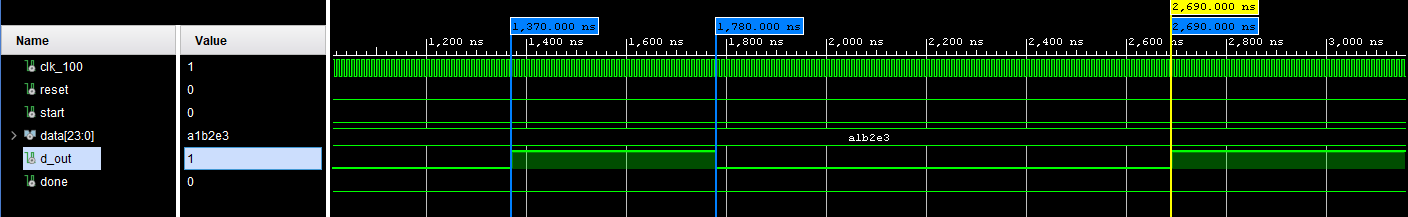
\includegraphics[scale=0.4]{driver_0_hibas.PNG}

\tab Látható, hogy nullás küldése esetén a kimenet \SI{0.41}{\micro\second}-ot van magas feszűltségen tartva \SI{0.45}{\micro\second} helyett és \SI{0.91}{\micro\second}-ot van
alacsony feszűltségen tartva, \SI{0.85}{\micro\second} helyett.

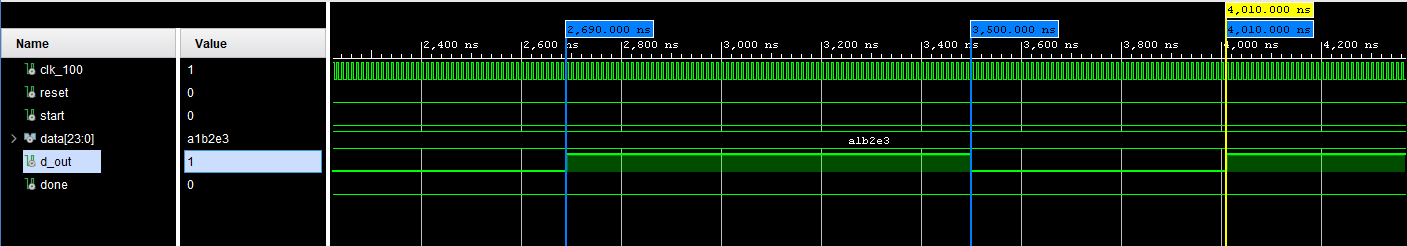
\includegraphics[scale=0.4]{driver_1_hibas.PNG}

\tab Itt látható, hogy 1-es küldése esetén a kimenet \SI{0.81}{\micro\second}-ot van magas feszűltésgen tartva \SI{0.8}{\micro\second} helyett és \SI{0.51}{\micro\second}-ot van
alacsony feszűltségen tartva, \SI{0.45}{\micro\second} helyett.

Ezt egyszerűen meg lehet oldani a ciklusszámok módosítása által.

Módosított ciklusszámok:

\begin{itemize}
\item Logikai 1-es
	\begin{itemize}
	\item 79 ciklus magas feszűltségen
	\item 39 ciklus alacsony feszűltségen
	\end{itemize}
\item Logikai 0-ás
	\begin{itemize}
	\item 39 ciklus magas feszűltségen
	\item 79 ciklus alacsony feszűltségen
	\end{itemize}
\end{itemize}

\tab A frissített értékekkel a WS2813 protokollja már pontosan be van tartva.

\tab Logikai egyesre:

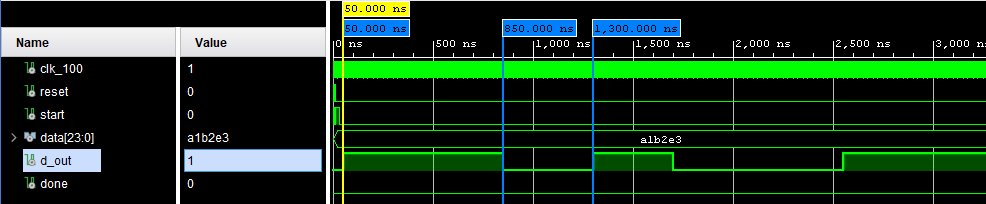
\includegraphics[scale=0.6]{driver_1_helyes.PNG}

\tab Logikai nullásra:

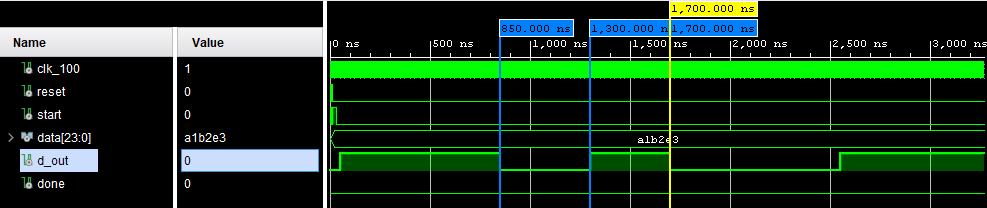
\includegraphics[scale=0.6]{driver_0_helyes.PNG}

\tab A másik két követelmény is teljesül:

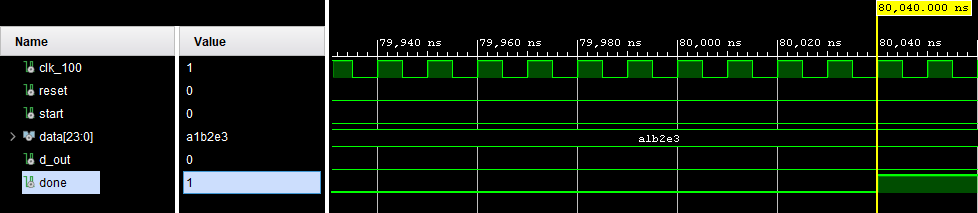
\includegraphics[scale=0.4]{driver_done.PNG}

\tab A 24 bit-es blokk elküldése után a done jel egyesre lett állítva és \SI{80.04}{\micro\second} alatt sikerült az egész 24 bit-es blokkot elküldeni.


\subsection{BRAM memória}

\tab A BRAM memóriák IP Catalog-ból lettek kigenerálva\cite{vhdlguru2010bram}. Kezdőértékek egy \textbf{coefficient} file-ból lettek feltöltve\cite{vhdlguru2010bramcoe}.
A \textbf{coefficient} file:
\begin{verbatim}
	memory_initialization_radix=16;
	memory_initialization_vector=00000A,00000B,00000C,00000D,
		00000E,00000F,000010,000011,000012,000013,000014,000015,000016,000017,000018,000019;
\end{verbatim}

A szimuláció eredménye:

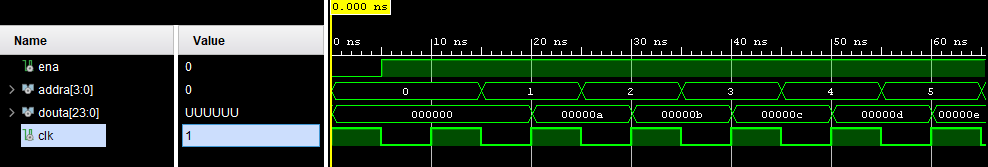
\includegraphics[scale=0.6]{bram_szimulacio.PNG}

\tab Megfigyelésem alapján a generált BRAM modul felfutó órajelre olvassa be a következő címet, és ugyanúgy felfutó órajelre teszi ki az adatot a kimenetre, de csak egy egész órajellel a cím beolvasása után.
